\section{Outputs and Results}

The complete system was implemented and tested in simulation. A demonstration video and all source code are linked on the title page. Below we present the key outputs.

\subsection{System Demonstration}

The teleoperation pipeline runs in real time: the operator holds the iPhone, starts the AR session, and moves the phone in 3D space. The UR10e model in RViz responds immediately, with end-to-end latency under 100~ms. Figure~\ref{fig:demo} shows the iOS app and RViz side by side during a teleoperation session.

% \begin{figure}[H]
%     \centering
%     \todo{Insert side-by-side screenshot: iOS app (left) and RViz (right) during teleoperation.}
%     \caption{System in operation. Left: iOS app showing the device pose matrix and feedback indicators. Right: RViz displaying the UR10e at the corresponding joint configuration.}
%     \label{fig:demo}
% \end{figure}

\begin{figure}[H]
    \centering
    \begin{minipage}{0.45\textwidth}
        \centering
        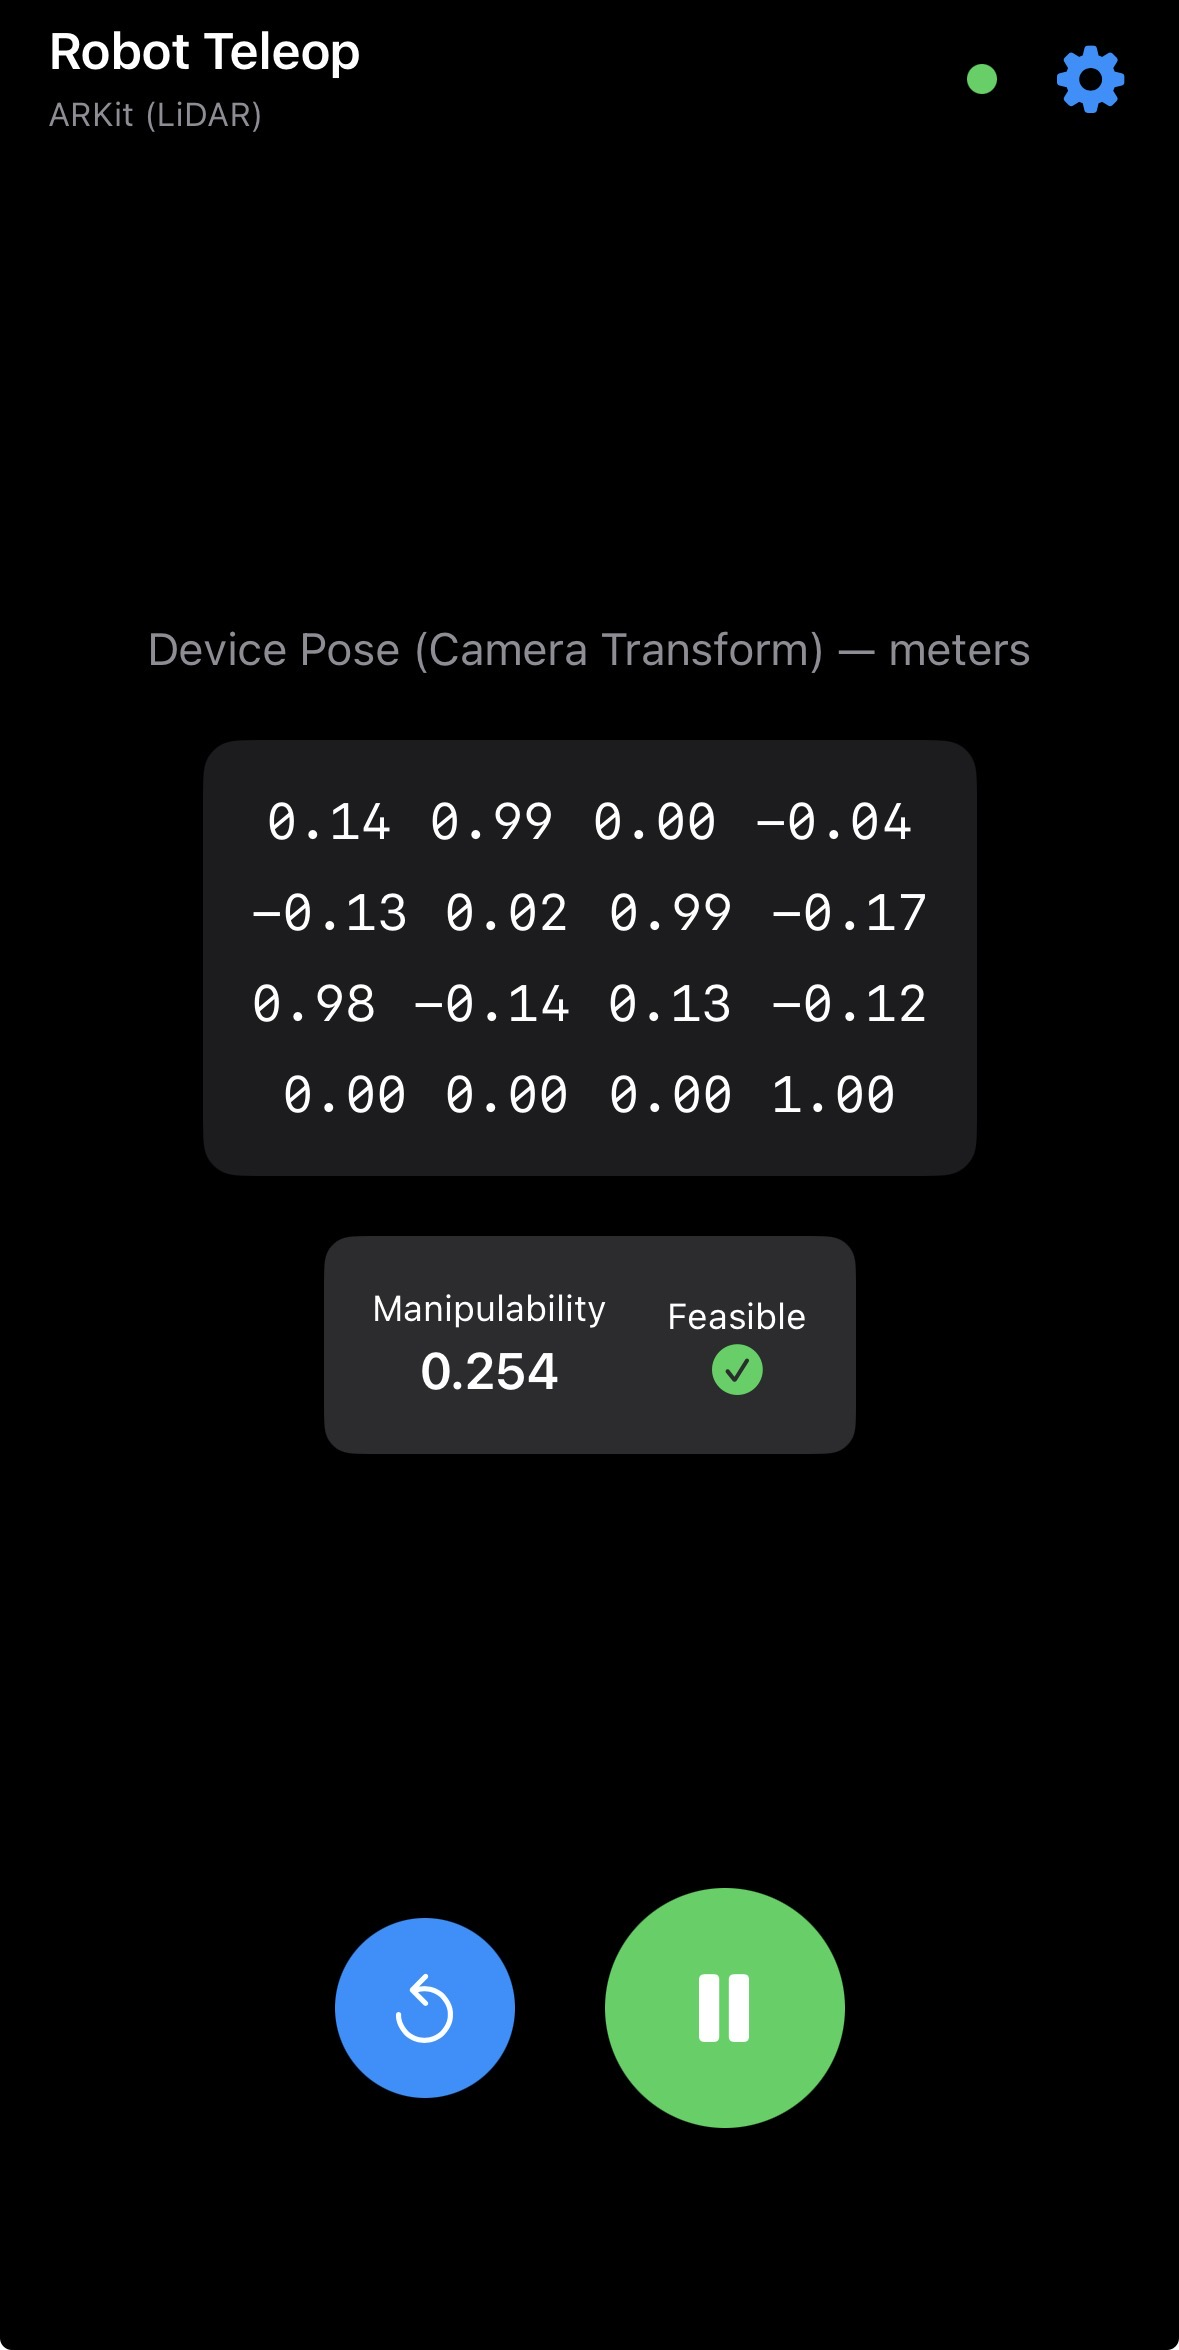
\includegraphics[width=0.5\linewidth]{imgs/phone_1.jpg}
    \end{minipage}\hfill
    \begin{minipage}{0.45\textwidth}
        \centering
        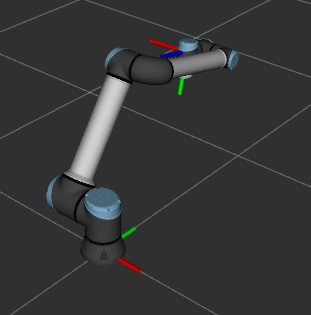
\includegraphics[width=0.8\linewidth]{imgs/rviz_1.png}
    \end{minipage}\\[2ex]
    \begin{minipage}{0.45\textwidth}
        \centering
        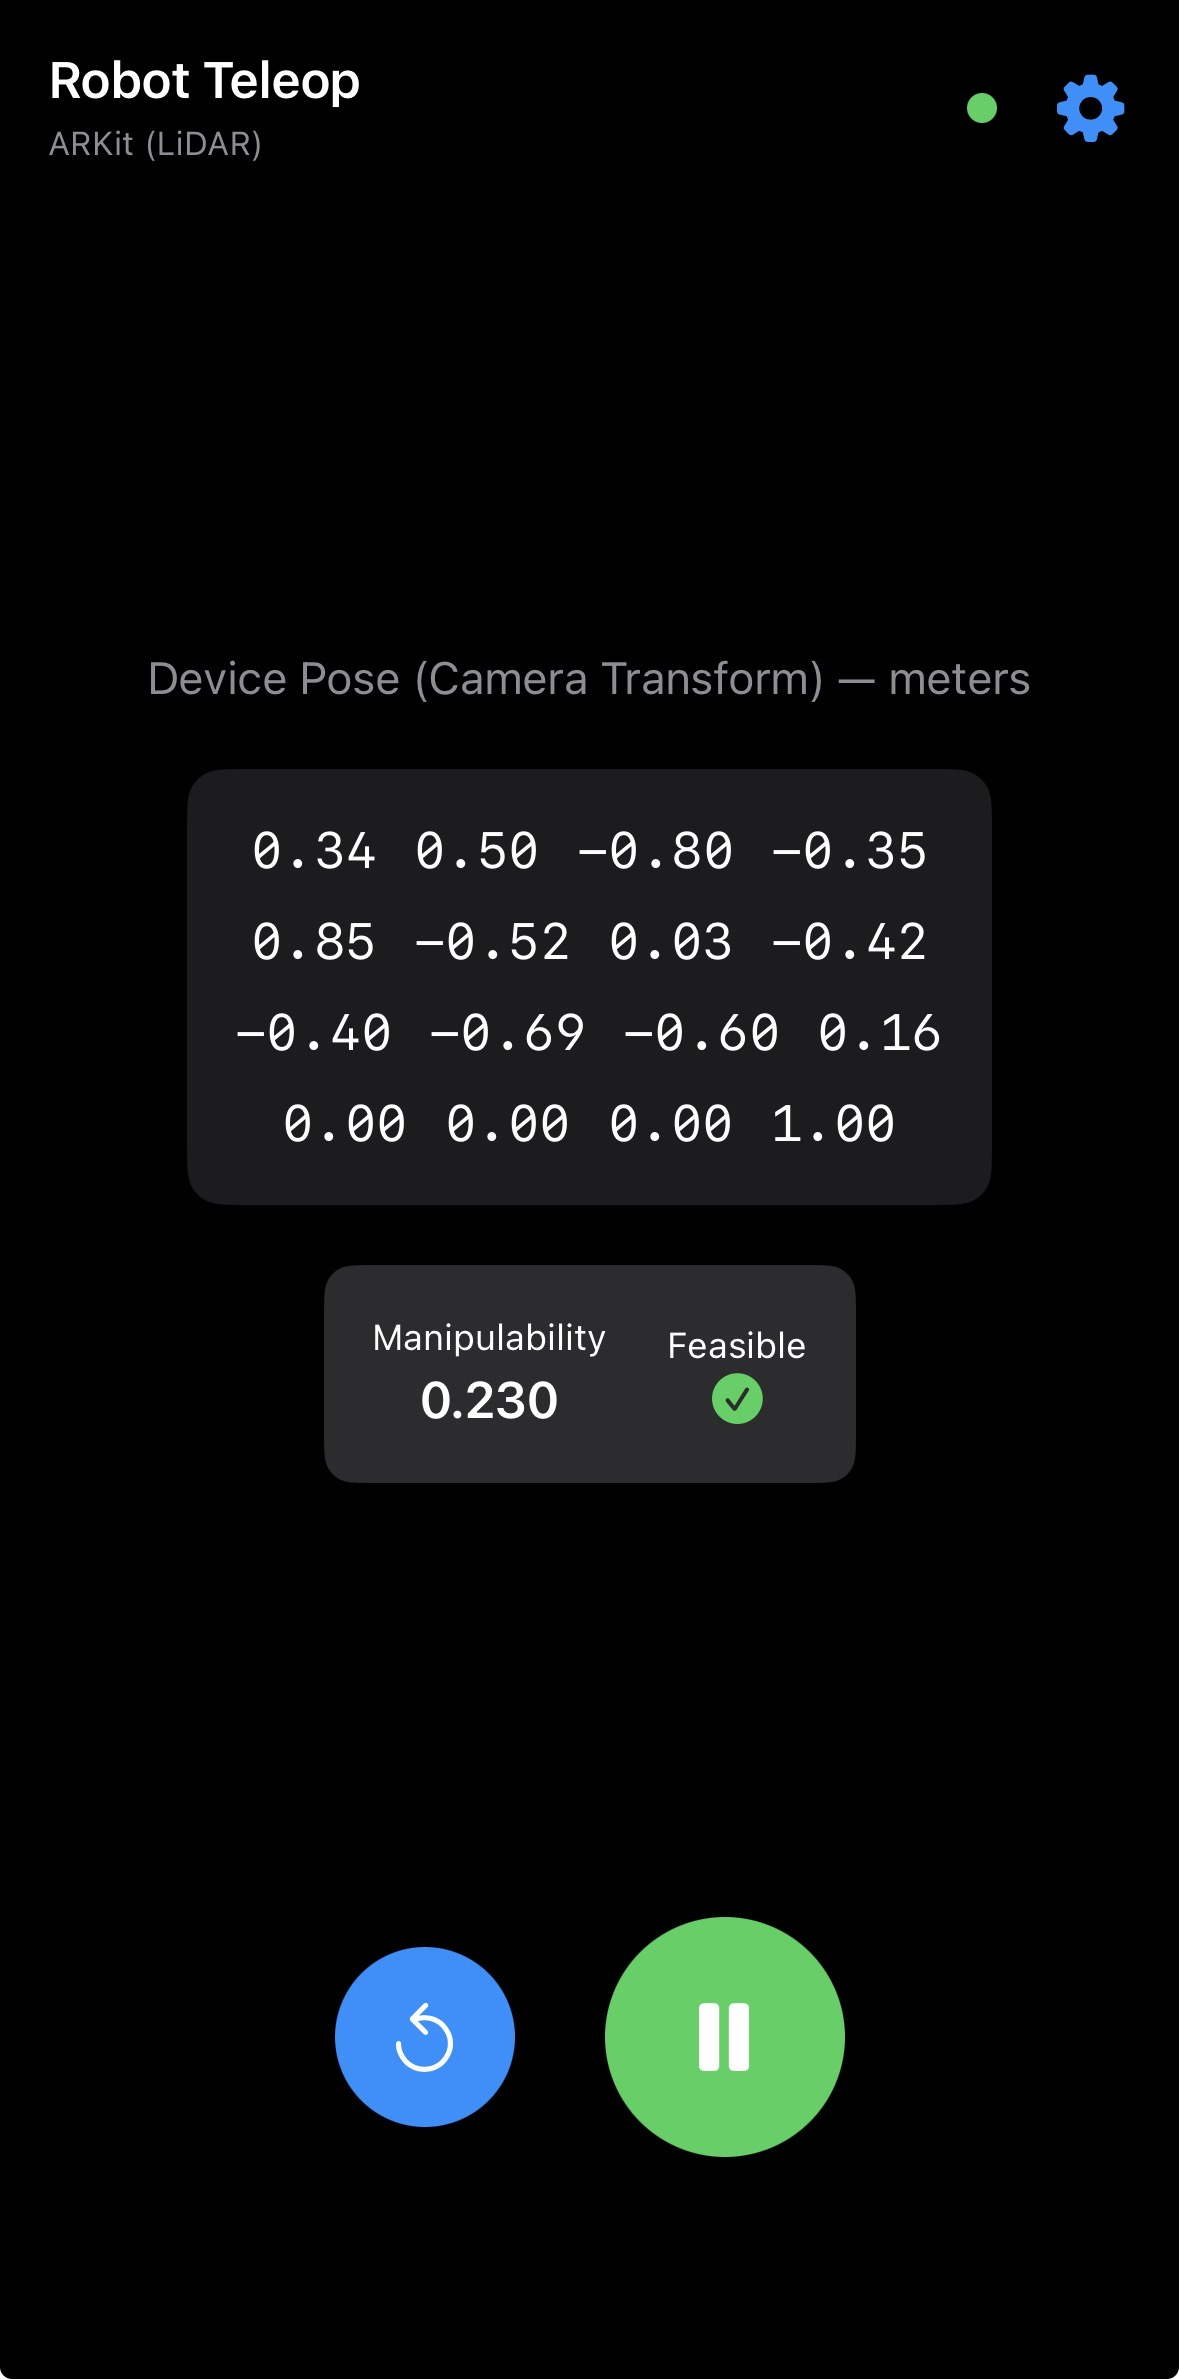
\includegraphics[width=0.5\linewidth]{imgs/phone_2.jpg}
    \end{minipage}\hfill
    \begin{minipage}{0.45\textwidth}
        \centering
        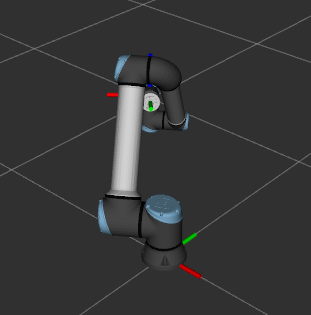
\includegraphics[width=0.8\linewidth]{imgs/rviz_2.png}
    \end{minipage}

    \vspace{2ex}
    \caption{System in operation. Left: iOS app showing the device pose matrix and feedback indicators. Right: RViz displaying the UR10e at the corresponding joint configuration.}
    \label{fig:demo}
\end{figure}

\subsection{Position Mode}

In position mode, the phone's relative displacement maps directly to a target end-effector pose via analytical IK. Figure~\ref{fig:pos_mode} shows joint trajectories during a position-mode session.

\begin{figure}[H]
    \centering
    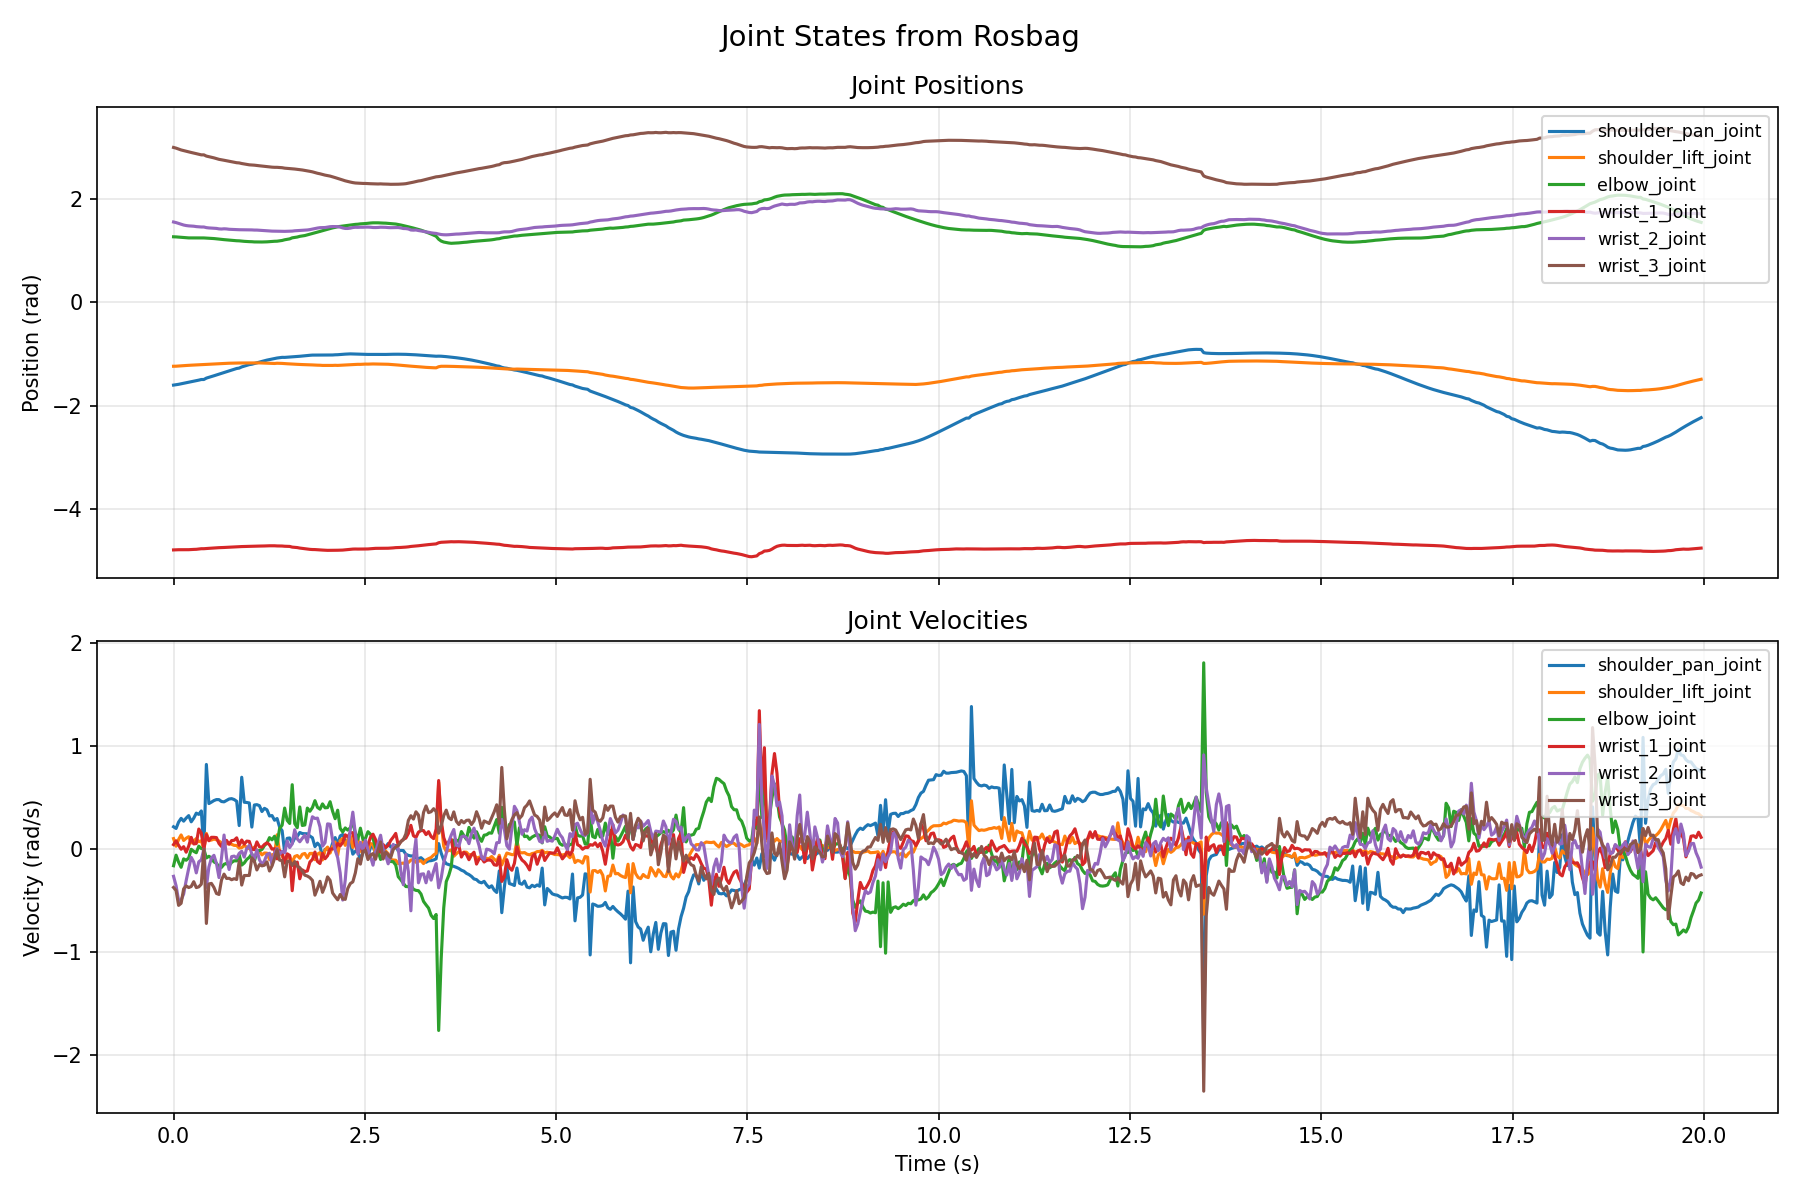
\includegraphics[width=0.8\linewidth]{imgs/pos_mode.png}
    \caption{Joint states during a position-mode teleoperation session.}
    \label{fig:pos_mode}
\end{figure}

In position mode, the elbow-up solution selection ensures continuous, physically plausible joint trajectories without configuration flips. However, the velocity is not smooth and there can still be sudden discontinuous jumps in joint position as can be seen around the 13s mark in Figure~\ref{fig:pos_mode}.

\subsection{Velocity Mode}

In velocity mode, the phone's twist drives the robot via resolved-rate control. Figure~\ref{fig:vel_mode} shows recorded joint positions and velocities during a velocity-mode session, captured via automatic rosbag recording. This maneuver was done to be similar of that of the position mode maneuever.

\begin{figure}[H]
    \centering
    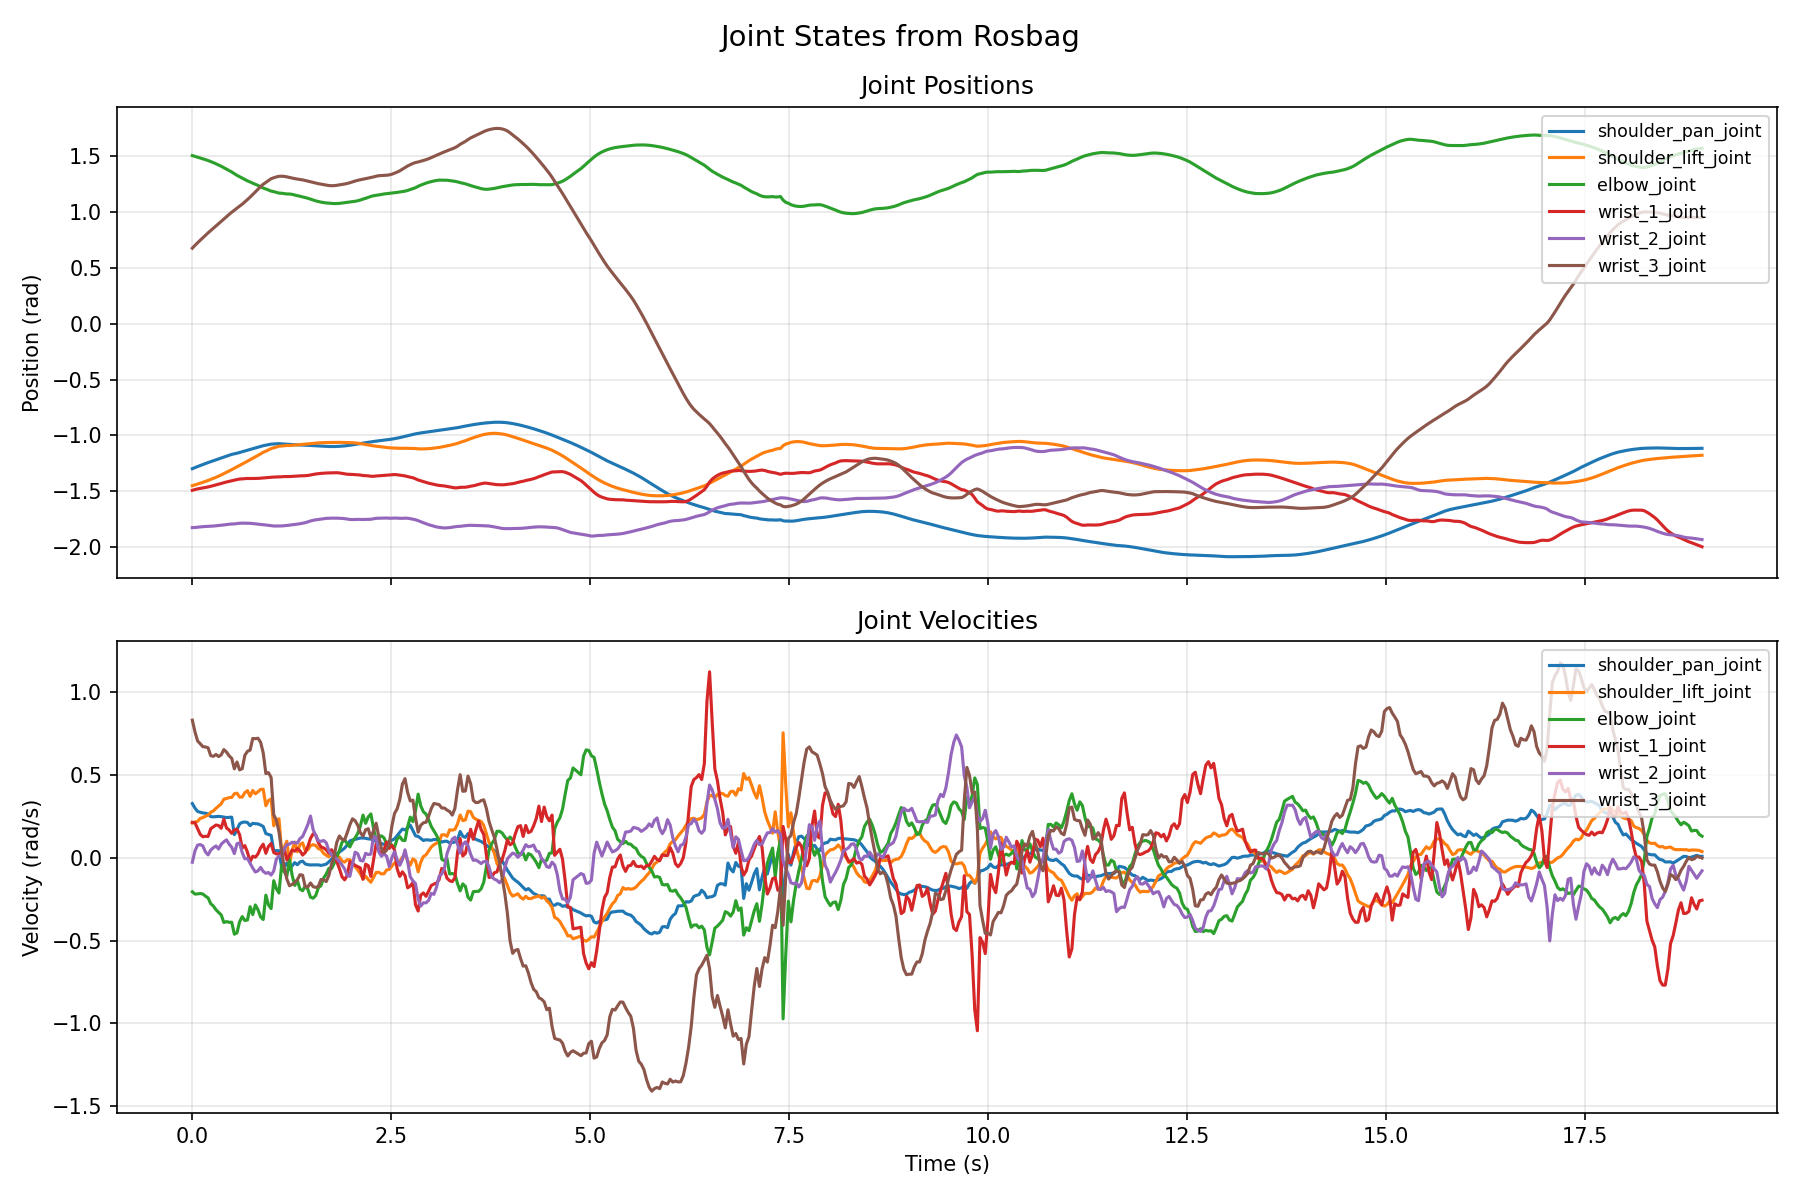
\includegraphics[width=0.8\linewidth]{imgs/vel_mode.png}
    \caption{Joint states during a velocity-mode teleoperation session.}
    \label{fig:vel_mode}
\end{figure}

% The adaptive damping is visible in the velocity traces: as the manipulator approaches singular configurations, joint velocities are attenuated rather than exhibiting the large spikes that would occur with an undamped pseudoinverse.

The smooth velocity profiles demonstrate the damped least-squares controller's singularity avoidance as well as the twist filtering. However, in velocity mode the robot's position tends to drift after doing a maneuver and then coming back to the starting position. This was observed with or without the twist filtering. 

\subsection{Reset Behavior}

Pressing the reset button on the iOS app sends a command that snaps the robot to the home configuration $\mathbf{q}_\text{home} = [-\pi/2,\, -\pi/2,\, \pi/2,\, -\pi/2,\, -\pi/2,\, 0]$ and re-references the phone's current pose. Figure~\ref{fig:reset} shows the joint positions before and after a reset event. When deploying this system to a physical robot, this feature would compute a smooth trajectory from the current state to the home state, to avoid unsafe jumps in the commanded joint positions.

\begin{figure}[H]
    \centering
    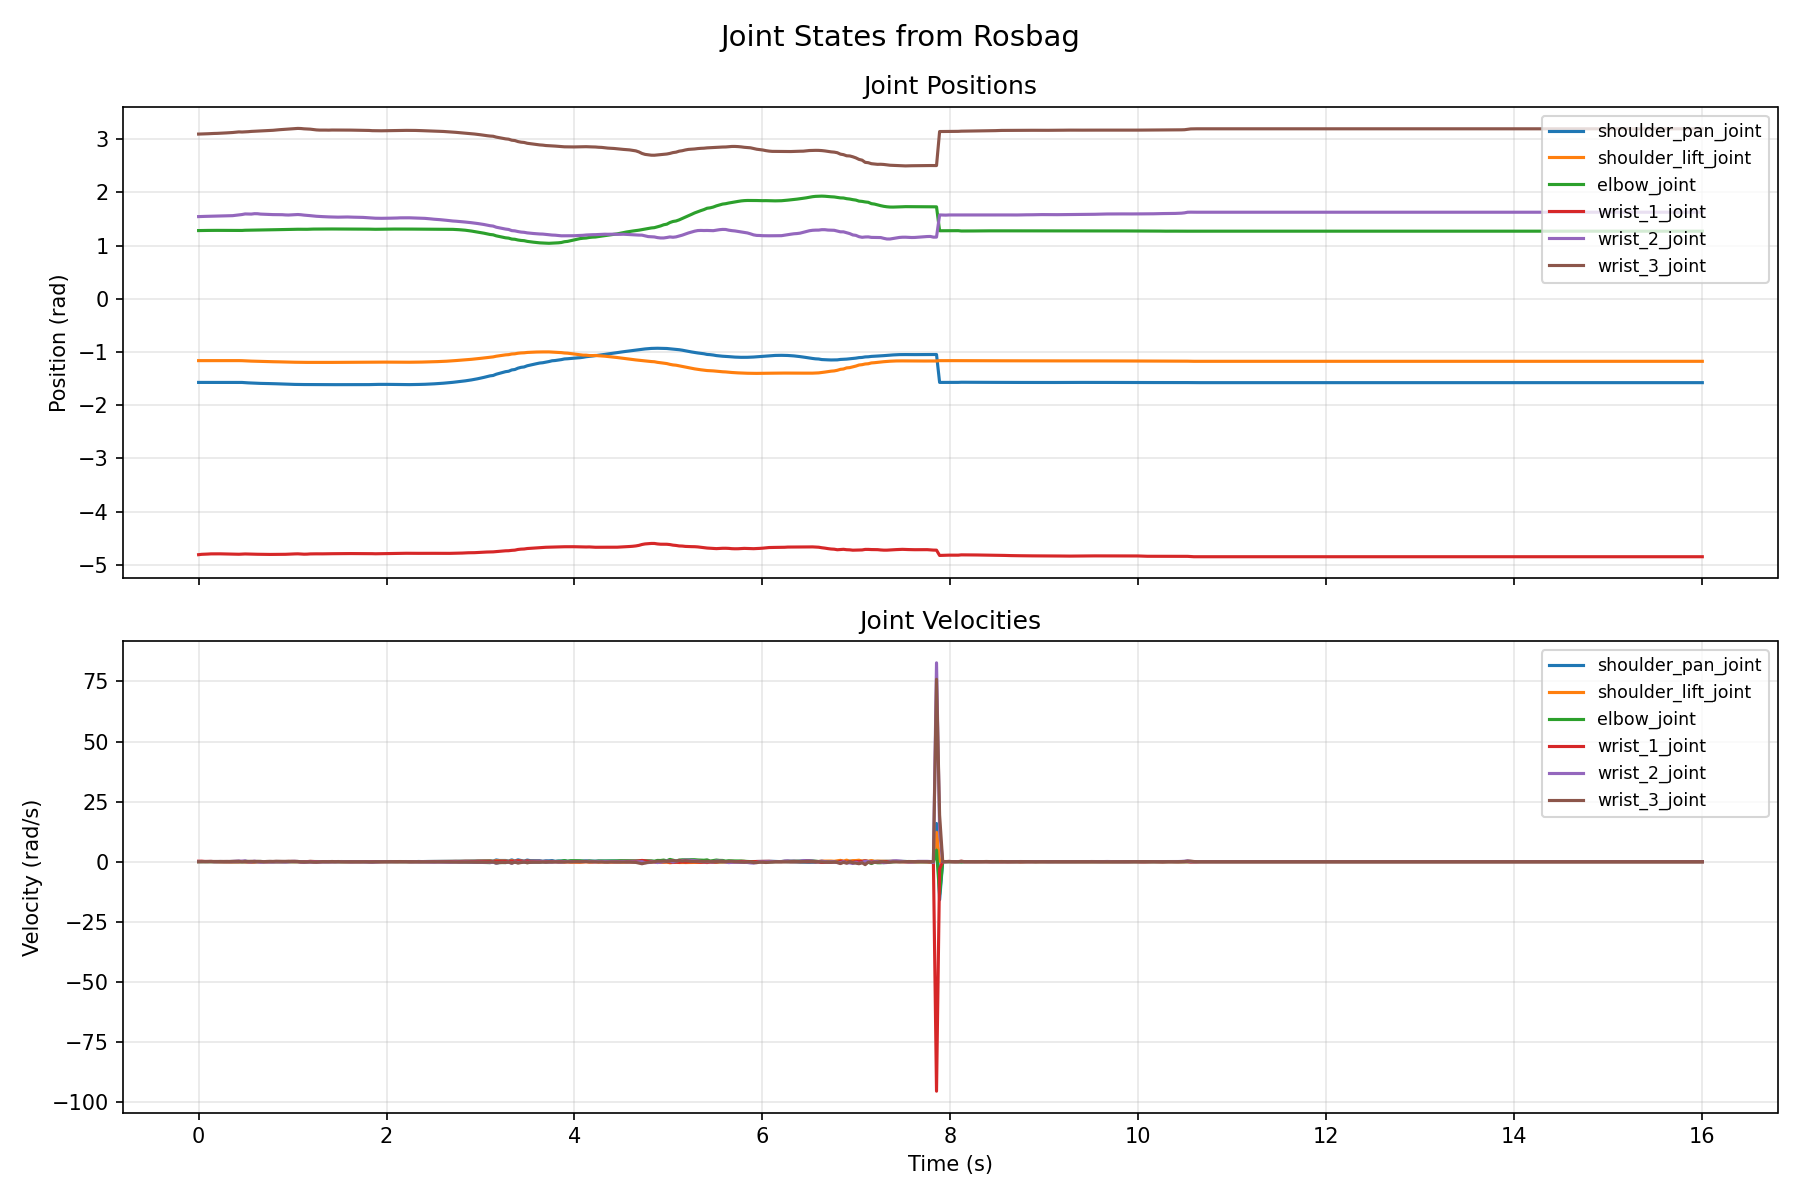
\includegraphics[width=0.8\linewidth]{imgs/reset.png}
    \caption{Reset event. The robot snaps to the home configuration, and subsequent phone movements are relative to the new reference pose.}
    \label{fig:reset}
\end{figure}

\subsection{Debug Dashboard}

A web-based debug dashboard provides real-time visualization of all system telemetry, including joint angles, manipulability, twist magnitude, and joint limit proximity. Figure~\ref{fig:dashboard} shows the dashboard during operation. We used this while in development to refine our system.

\begin{figure}[H]
    \centering
    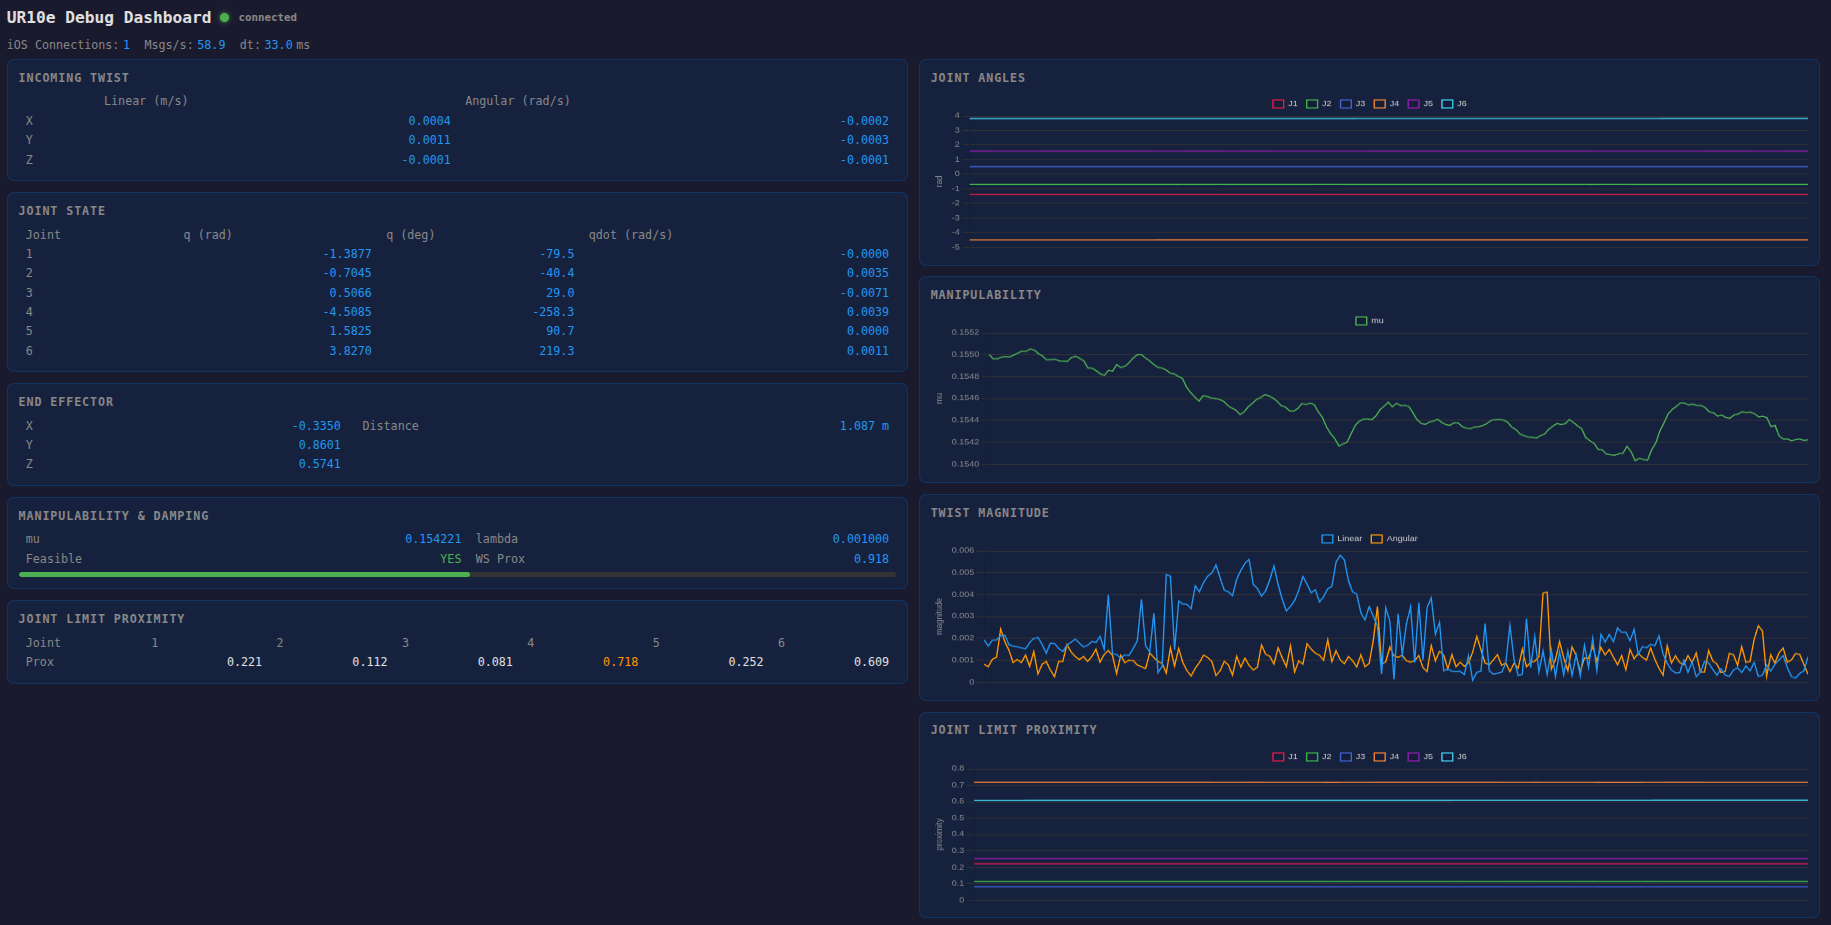
\includegraphics[width=1\linewidth]{imgs/dashboard.png}
    \caption{Web debug dashboard showing live telemetry: joint state table, end-effector position, manipulability bar, and time-series charts for joint angles, manipulability, twist magnitude, and joint limit proximity.}
    \label{fig:dashboard}
\end{figure}
